\documentclass[]{report}

\voffset=-1.5cm
\oddsidemargin=0.0cm
\textwidth = 480pt

\usepackage{framed}
\usepackage{subfiles}
\usepackage{graphics}
\usepackage{newlfont}
\usepackage{eurosym}
\usepackage{amsmath,amsthm,amsfonts}
\usepackage{amsmath}
\usepackage{color}
\usepackage{amssymb}
\usepackage{multicol}
\usepackage[dvipsnames]{xcolor}
\usepackage{graphicx}
\begin{document}
\section{Statistics for grouped data}
Grouped data refers to the arrangement of raw data with a wide range of values into groups. This process makes the data more manageable. Graphs and frequency diagrams can then be drawn showing the class intervals chosen instead of individual values.


\noindent An estimate, $\bar{x}$, of the mean of the population from which the data are drawn can be calculated from the grouped data as:
\[ \bar{x} = \frac{\sum f x }{\sum f}\]
In this formula, $x$ refers to the mid-point of the class intervals, and $f$ is the class frequency. Note that the result of this will be different from the sample mean of the ungrouped data.


\begin{tabular}{|c|c|c|}
	\hline
	Class limits& Class midpoint & frequency \\
	\hline
	\$240 - 259.99 & \$250 &7\\
	\$260 - 279.99 & \$270 &20\\
	\$280 - 299.99 & \$290 &33\\
	\$300 - 319.99 & \$310 &25\\
	\$320 - 339.99 & \$330 &11\\
	\$340 - 359.99 & \$350 &4\\
	\hline
	& & Total = 100\\
	\hline
\end{tabular}

\subsection{Cumulative frequency}
The graph of a cumulative frequency distribution is called an ogive (pronounced ``o-jive"). For the less-than
type of cumulative distribution, this graph indicates the cumulative frequency below each exact class limit of
the frequency distribution. When such a line graph is smoothed, it is called an ogive curve.


\subsection{Relative frequency}
\begin{itemize}
	\item A relative frequency distribution is one in which the number of observations associated with each class has
	been converted into a relative frequency by dividing by the total number of observations in the entire
	distribution. 
	\item Each relative frequency is thus a proportion, and can be converted into a percentage by multiplying
	by 100.\item One of the advantages associated with preparing a relative frequency distribution is that the cumulative
	distribution and the ogive for such a distribution indicate the cumulative proportion (or percentage) of
	observations up to the various possible values of the variable. A percentile value is the cumulative percentage of
	observations up to a designated value of a variable.
\end{itemize}





\noindent \textbf{Measures of Centrality}

\begin{itemize}
	\item Measures of centrality give one representative number for the location of the centre of the distribution of data.
	\item
	The most common measures are the \textbf{\emph{mean}} and the \textbf{\emph{ median }}.
	\item We must make a distinction between a sample mean and a population mean: The sample mean is simply the average of all the items in a sample.  \item The population mean (often represented by the Greek letter $\mu$) is simply the average of all the items in a population. \item Because a population is usually very large, the population mean is usually an unknown constant.
	\item We will return to the matter of population means in due course. For now, we will look at sample means.
\end{itemize}


\noindent \textbf{Sample Mean}

\begin{itemize}
	\item The sample mean is an estimator available for estimating the population mean . It is a measure of location, commonly called the average, often denoted $\bar{x}$, where $x$ is the data set.
	\item
	Its value depends equally on all of the data which may include outliers. It may not appear representative of the central region for skewed data sets.
	\item
	It is especially useful as being representative of the whole sample for use in subsequent calculations.
	\item The sample mean of a data set is defined as :
	\[ \bar{x} = { \sum x_i\over n}\]
	\item $\sum x_i$ is the summation of al the elements of $x$, and $n$ is the sample size.
\end{itemize}

\noindent \textbf{Computing the sample mean}

Suppose we roll a die 8 times and get the following scores: $x = \{ 5, 2, 1, 6, 3, 5, 3, 1\}$ \\ \bigskip

What is the sample mean of the scores $\bar{x}$?
\[ \bar{x}  = {5 + 2 +  1 +  6 +  3 +  5 +  3 +  1 \over 8 } = {26 \over 8} =  3.25 \]




\noindent \textbf{Using \texttt{R} to compute mean (and median)}
When implementing this in R, we would use the following code

\begin{verbatim}
> # create the "vector" x with the required values
> x=c(5, 2, 1, 6, 3, 5, 3, 1)
>
> mean(x)
[1] 3.25
>
> # See next slides first.
> sort(x)
[1] 1 1 2 3 3 5 5 6
> median(x)
[1] 3
\end{verbatim}


\noindent \textbf{Median}
\begin{itemize}
	\item The other commonly used measure of centrality is the median.
	
	\item The median is the value halfway through the ordered data set, below and above which there lies an equal number of data values.
	\item For an odd sized data set, the median is the middle element of the \textbf{ordered} data set.
	\item For an even sized data set, the median is the average of the middle pair of elements of an \textbf{ordered} data set.
	\item It is generally a good descriptive measure of the location which works well for \textbf{\emph{skewed data}}, or data with \textbf{\emph{outliers}}.
	
	\item For later, the median is the 0.5 quantile, and the second quartile $Q_2$.
\end{itemize}


\noindent \textbf{Computing the median}
\textbf{Example:}


With an odd number of data values, for example nine, we have:
\begin{itemize}
	\item Data : $\{96, 48, 27, 72, 39, 70, 7, 68, 99 \}$
	\item Ordered Data :  $\{7, 27, 39, 48, 68, 70, 72, 96, 99\}$
	\item Median : 68, leaving four values below and four values above
\end{itemize}
\bigskip
With an even number of data values, for example 8, we have:
\begin{itemize}
	\item Data : $\{96, 48 ,27 ,72, 39, 70, 7, 68  \}$
	\item Ordered Data : $\{7, 27, 39, 48, 68, 70, 72, 96\}$
	\item Median : Halfway between the two 'middle' data points - in this case halfway between 48 and 68, and so the median is 58
\end{itemize}

\noindent \textbf{Using \texttt{R} to compute mean (and median)}
When implementing this in R, we would use the following code

\begin{verbatim}
> x1=c(96, 48, 27, 72, 39, 70, 7, 68, 99 )
> sort(x1)
[1]  7 27 39 48 68 70 72 96 99
> median(x1)
[1] 68
>
> x2=c(96, 48 ,27 ,72, 39, 70, 7, 68)
> sort(x2)
[1]  7 27 39 48 68 70 72 96
> median(x2)
[1] 58
\end{verbatim}


%--------------------------------------------------------%

\noindent \textbf{Dispersion }

\begin{itemize}
	\item The data values in a sample are not all the same. This variation between values is called \textbf{ \emph{dispersion}}.
	
	\item When the dispersion is large, the values are widely scattered; when it is small they are tightly clustered.
	
	%The width of diagrams such as dot plots, box plots, stem and leaf plots is greater for samples with more dispersion and vice versa.
	
	\item
	There are several measures of dispersion, the most common being the variance and  standard deviation. These measures indicate to what degree the individual observations of a data set are dispersed or 'spread out' around their mean.
	
	\item
	In engineering and science, high precision is associated with low dispersion.
\end{itemize}

\noindent \textbf{Range}

\begin{itemize}
	\item The range of a sample (or a data set) is a measure of the spread or the dispersion of the observations. \item It is the difference between the largest and the smallest observed value of some quantitative characteristic and is very easy to calculate.
	
	\item A great deal of information is ignored when computing the range since only the largest and the smallest data values are considered; the remaining data are ignored.
	
	\item The range value of a data set is greatly influenced by the presence of just one unusually large or small value in the sample (outlier).
\end{itemize}

\textbf{Example}


The range of $\{65,73,89,56,73,52,47\}$ is $ 89-47 = 42$.

% If the highest score in a 1st year statistics exam was 98 and the lowest 48, then the range would be 98-48 = 50.


Consider the three data sets $X$, $Y$ and $Z$
\begin{itemize}
	\item $X= \{900,925,950,975,1025,1050,1075,1100 \}$
	\item $Y=\{900,905,910,920,1080,1090,1095,1100\}$
	\item $Z=\{900,985,990,995,1005,1010,1015,1100\}$
\end{itemize}

For each of the data sets, the following statements can be verified

\begin{itemize}
	\item The mean of each data set is 1000
	\item There are 8 elements in each data set
	\item The minima and maxima are 900 and 1100 for each set
	\item The range is 200.
\end{itemize}

From the plot on the next slide, notice how different the three data sets are in terms of dispersion around the mean value.



%--------------------------------------------------------%


\noindent \textbf{Introducing Variance}


%\begin{center}
%	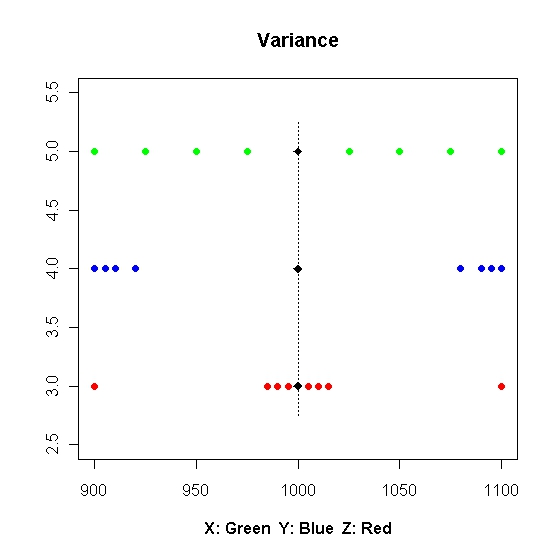
\includegraphics[scale=0.4]{images/2AVariance}
%\end{center}


%--------------------------------------------------------%

\noindent \textbf{Variance}


\begin{itemize}
	
	\item The (population) variance of a random variable is a non-negative number which gives an idea of how widely spread the values are likely to be; the larger the variance, the more scattered the observations on average.
	
	\item Stating the variance gives an impression of how closely concentrated round the expected value the distribution is; it is a measure of the 'spread' of a distribution about its average value.
	
	\item We distinguish between population variance (denoted $\sigma^2$) and sample variance (denoted $s^2$). For now, we will look only at sample variance.
	
\end{itemize}


\begin{itemize}
	\item Now consider an experiment with only two outcomes. Independent repeated trials of such an experiment are
	called Bernoulli trials, named after the Swiss mathematician Jacob Bernoulli (1654–1705). \item The term \textbf{\emph{independent
			trials}} means that the outcome of any trial does not depend on the previous outcomes (such as tossing a coin).
	\item We will call one of the outcomes the ``success" and the other outcome the ``failure".
\end{itemize}


%=================================================================== %

\begin{itemize} \item
	Let $p$ denote the probability of success in a Bernoulli trial, and so $q = 1 - p$ is the probability of failure.
	A binomial experiment consists of a fixed number of Bernoulli trials. \item A binomial experiment with $n$ trials and
	probability $p$ of success will be denoted by
	\[B(n, p)\]
\end{itemize}

%=================================================================== %



	
\section{Cumulative frequency}
The graph of a cumulative frequency distribution is called an ogive (pronounced ``o-jive"). For the less-than
type of cumulative distribution, this graph indicates the cumulative frequency below each exact class limit of
the frequency distribution. When such a line graph is smoothed, it is called an ogive curve.


\section{Relative frequency}
\begin{itemize}
	\item A relative frequency distribution is one in which the number of observations associated with each class has
	been converted into a relative frequency by dividing by the total number of observations in the entire
	distribution. 
	\item Each relative frequency is thus a proportion, and can be converted into a percentage by multiplying
	by 100.\item One of the advantages associated with preparing a relative frequency distribution is that the cumulative
	distribution and the ogive for such a distribution indicate the cumulative proportion (or percentage) of
	observations up to the various possible values of the variable. A percentile value is the cumulative percentage of
	observations up to a designated value of a variable.
\end{itemize}



\section{Statistics for grouped data}
Grouped data refers to the arrangement of raw data with a wide range of values into groups. This process makes the data more manageable. Graphs and frequency diagrams can then be drawn showing the class intervals chosen instead of individual values.


\noindent An estimate, $\bar{x}$, of the mean of the population from which the data are drawn can be calculated from the grouped data as:
\[ \bar{x} = \frac{\sum f x }{\sum f}\]
In this formula, $x$ refers to the mid-point of the class intervals, and $f$ is the class frequency. Note that the result of this will be different from the sample mean of the ungrouped data.


\begin{tabular}{|c|c|c|}
	\hline
	Class limits& Class midpoint & frequency \\
	\hline
	\$240 - 259.99 & \$250 &7\\
	\$260 - 279.99 & \$270 &20\\
	\$280 - 299.99 & \$290 &33\\
	\$300 - 319.99 & \$310 &25\\
	\$320 - 339.99 & \$330 &11\\
	\$340 - 359.99 & \$350 &4\\
	\hline
	& & Total = 100\\
	\hline
\end{tabular}

\end{document}